
En esta etapa, se procede a recolectar todos los datos análogos y digitales con los que cuenta en CA-SENA-POP, para almacenarlos de manera digital y proceder a analizar los datos mediante algoritmos en Matlab y/o Python. Es importante recalcar que para ambos software se requiere una estructura de datos en tablas debidamente organizadas, ya sea para tratarlos como $dataframes$, matrices, arreglos, o como tablas de archivos $^{*}.csv$.

\section{Recolección de datos} \label{datarecol}

Tal y como se mencionó en el capítulo anterior, los datos referentes a Peso, Leche y Alimentación, de cada una de las reses del CA-SENA-POP se encuentran registradas de manera física o digital; ya sea en hojas impresas como el ejemplar de la figura \ref{regleche1png}, así como también en bases de datos digitales como el de la figura \ref{tauruspng}. No obstante, estos datos \textbf{no} pueden ser importados directamente a algún software de procesamiento de datos. Esto puesto que para los datos físicos, se tienen algunas barreras y/o inconvenientes externos tales como los diferentes tipos de letra,  el estado físico de las paginas, y la diferencia entre los números de un ente registrado u otro; mientras que para los datos digitales, estos se encuentran almacenados en el software de pago de manera privada, siendo datos protegidos de acuerdo a la ley de ``Habeas data'', por lo que no pueden ser exportados directamente para manipulación del público.\\ % Feb  2023

% \subsection{Registros de ``Leche''}
Teniendo en cuenta que los datos de producción lechera se registran de manera manual, esta tarea es llevada a cabo por distintas personas. Desde aprendices hasta instructores y supervisores; por lo tanto, los datos son escritos por distintas personas, que manejan distintos tipos de letra, distinto orden, distintas practicas adecuadas de escritura, entre otras. Esto implica que los números registrados en las paginas físicas varíen de un tipo de letra a otra y deban ser analizados o copiados rigurosamente de manera digital. Además, es importante mencionar, que estas carpetas físicas de registro de datos, son expuestas a la intemperie, por lo que algunos registros han sido vulnerables ante lluvias, o sustancias que alteran el estado de la hoja de papel, dificultando así su interpretación a primera vista.\\

Es importante hacer esta observación, dado que por estas mismas circunstancias, \textbf{no} es posible extraer los datos de las tablas mediante algoritmos de inteligencia artificial de procesamiento de imágenes de manera consistente, pues estos datos pueden ser fácilmente tergiversados o malinterpretados como los ejemplares de la figura \ref{datosamanopng}.

\begin{figure}[H]
	 \begin{center}
	 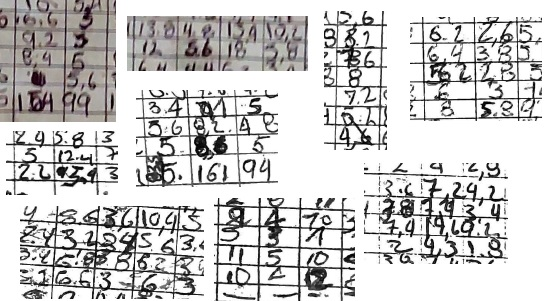
\includegraphics[scale=1.05]{img/datosamano.jpg}
	 \end{center}
	 \caption{Ejemplares de datos físicos con malas prácticas de escritura. \label{datosamanopng}}
\end{figure}

En cuanto a los registros de peso, dado que la cantidad de datos no es tan abrumadora a comparación de los registros de leche, estos datos son transcritos a archivos de excel y posteriormente a archivos con extensión $^{*}.csv$.

\section{Digitalización de los datos de producción lechera}

Teniendo en cuenta la descripción anterior, los datos fueron escaneados y posteriormente fueron transcritos de manera individual. Los datos utilizados en este trabajo consisten en los registros de producción lechera de distintas vacas que han entrado y salido de la producción ganadera, ya sea por motivos de compraventa, ingreso a gestación, salida por periodo de secado,  enfermedad, deceso, edad o cantidad de partos.\\

Los datos aquí utilizados comprenden fechas desde el 31 de Diciembre de 2018, hasta el 24 de Julio de 2022. En total se transcribieron de forma manual un total de $85.932$  datos, de los cuales, $37.956$ son datos numéricos representativos que pueden usarse para procesamiento de datos. Los $47.976$ datos restantes son datos categóricos que representan periodos de secado, horra, datos inexistentes o ilegibles, o registros desconocidos clasificados como datos NAN. Se cuenta con un total de 4 archivos pdf, en donde se almacenan los escaneos de los datos que comprenden esas fechas ya mencionadas.\\

Esta tarea de transcripción de datos tomó un tiempo aproximado de 1 semana;7 días, en jornadas de 8 horas cada día. Los datos que poseían dificultades de lectura e interpretación fueron corroborados con base en los datos de producción diaria neta y producción neta individual de cada vaca, datos existentes en las tablas escaneadas; por lo que se reduce el riesgo de transcripción de datos erróneos por causas humanas.

Aún sí existiese algún dato atípico o dato erróneo, esto puede corroborarse con la estructuración de los datos que se empleó para su análisis y que se explica en la sección a continuación.

\section{Reestructuración de los datos de leche}\label{reestructleche}
% \section{Datos de leche}
Una vez que se transcribieron los datos de manera individual para cada vaca. se procede a agrupar los datos en un archivo de excel organizado de la siguiente forma:

\subsection{Reestructuración inicial}

\begin{figure}[H]
	 \begin{center}
	 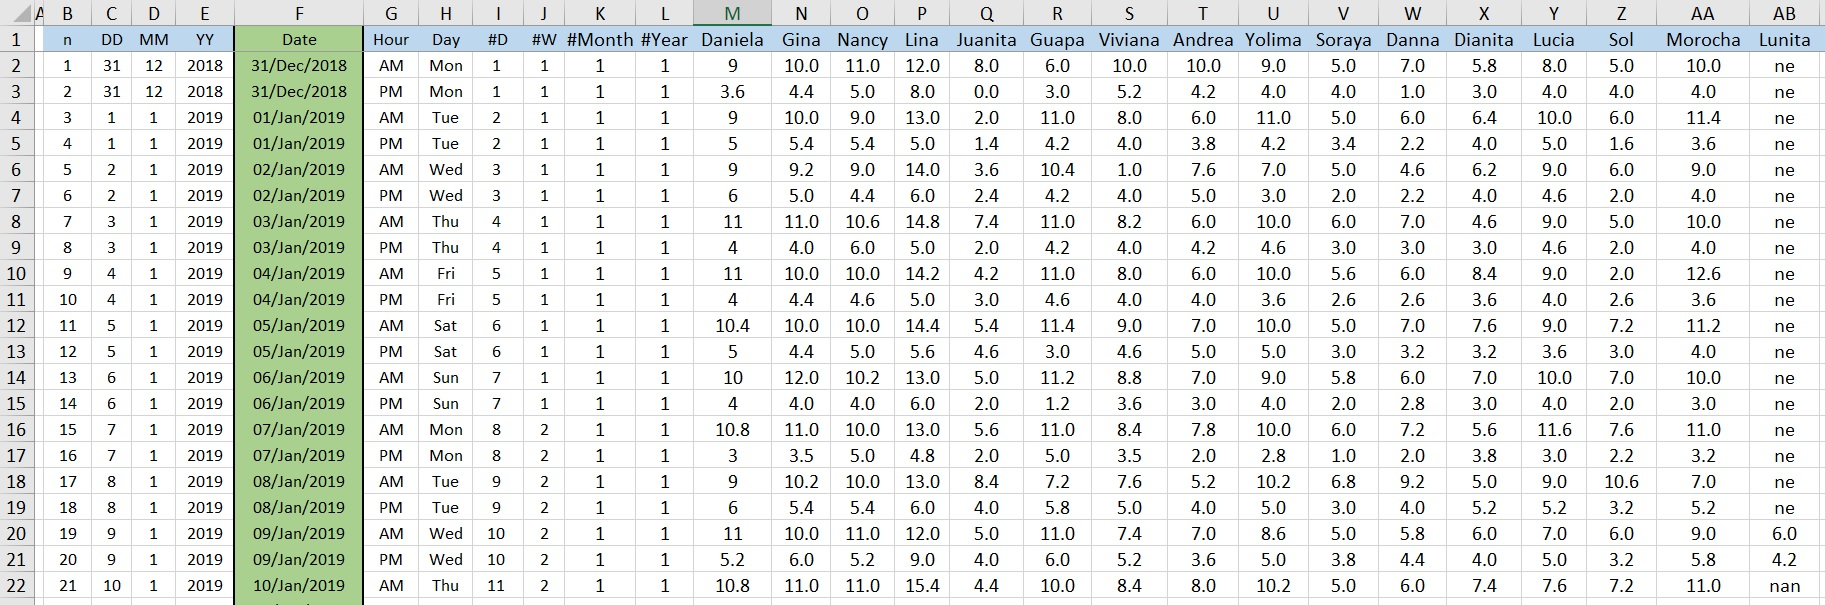
\includegraphics[scale=0.335]{img/dfinicial.jpg}
	 \end{center}
	 \caption{Reestructuración inicial de los datos de producción de leche transcritos. \label{dfinicialpng}}
\end{figure}

\begin{itemize}
    \item Cada fila, representa una \textbf{muestra - n} tomada en una \textbf{fecha (``DD/MM/AAAA'')} en una \textbf{franja horaria (AM o PM)}, en un \textbf{día de la semana (DAY y \#D)}, en una \textbf{semana (\#W)} , en un \textbf{mes (\#Month)} y en un \textbf{año (\#Year)} específico.
    \item Cada columna, representa una \textbf{vaca} que produjo una \textbf{cantidad de leche (valor numérico positivo)}.
    \item Cada 2 filas se tiene un cambio de fecha, pues se registran los datos de la mañana (AM) y también se registran los datos de la tarde (PM) como muestras separadas; más no como días distintos. Por lo tanto se tienen 2 muestras por cada día.
    \item En caso que una vaca no se encontrase en los registros de producción de leche para una fecha especifica y sus días anteriores, se cataloga como \textbf{vaca no existente} o \textbf{ne}
    \item En caso que una vaca muriera, los datos subsiguientes a esa fecha serán datos de tipo texto representados con la letra \textbf{M}.
    \item En caso que una vaca se vendiera,  los datos subsiguientes a esa fecha serán datos de tipo texto representados con la letra \textbf{V}.
    \item En caso que una vaca se encontrase en periodo de Horra,  los datos subsiguientes a esa fecha serán datos de tipo texto representados con la letra \textbf{H}, hasta indicado lo contrario.
    \item En caso que una vaca no se encontrase en periodo determinado, fuera por falta de preñes, horra, u otro motivo desconocido,  los datos subsiguientes a esa fecha aproximada serán datos de tipo texto representados con las letras \textbf{UL}, haciendo referencia a ``Unknown-Location''.
    \item En caso que una vaca se encontrase en periodo de secado, los datos subsiguientes a esa fecha serán datos de tipo texto representados con la letra \textbf{S}, hasta que se reincorpore tras el periodo de secado o hasta que se avise lo contrario (Muerte, Venta, Horra).
    \item En caso que un registro de producción de leche no haya sido transcrito, ya sea por malas practicas de escritura del documento físico, datos ilegibles o datos inexistentes, la casilla tendrá un valor de texto representado con las letras \textbf{NAN}, \textbf{haciendo referencia a un dato desconocido o dato inexistente por motivo desconocido}.
    \item En caso de tener valores numéricos 0, este valor es dejado como 0, si se muestra reincidencia en los días subsiguientes (suele suceder en fechas cercanas al periodo de secado), este valor será dejado así pues desde la práctica de toma de datos se ha considerado como una extracción de una cantidad de leche aproximadamente nula. No obstante, ya se ha mencionado que el dominio de los valores númericos de producciones de leche son \textbf{enteros positivos}.
    \item De las observaciones anteriores es importante agregar que los datos numéricos no pueden ser negativos.
    \item Se tiene un total de 2604 muestras para cada vaca, ya sea numérico o categórico. Se hace así pues las columnas de la matriz deben tener la misma cantidad de datos
    \item Se obtuvieron muestras de un total de 33 vacas distintas.
    \item Se maneja el dato desconocido con la denominación NAN y no con otro símbolo como el signo de interrogación ``?'', por motivos de formato al momento de transcribir los datos a Microsoft Excel.
\end{itemize}

\subsection{``Debugging'' y verificación de datos}

Como la transcripción de los datos se realiza de forma manual, existe el riesgo de añadir error humano a mediciones que ya cuentan con errores de medición y escritura. Para disminuir este error de transcripción, se verificó uno a uno los valores, antes, durante y después del proceso de transcripción. No obstante puede que se hayan pasado valores por alto como reflejo de un error humano.\\

Para ello, una vez obtenida la matriz agrupada en Excel, se verifican los tipos de datos y se corrobora que la cantidad neta de cada grupo sumen la cantidad total de datos. En caso contrario, el valor en cuestión se puede identificar el índice de la(s) muestra(s) no identificada(s) y mediante la fecha en la que fue(ron)  tomada(s), se puede corroborar tanto en la tabla de Excel, como en los archivos pdf escaneados. 

\subsection{Reestructuración numérica}

Notese que en la reestructuración inicial se puede observar que los datos pueden ser numéricos o categóricos, no obstante esto dificulta su análisis matricial en el software de Matlab por lo que se procede a tener algunas consideraciones adicionales.

\begin{itemize}
    \item En caso de muerte o venta, se considera como dato de valor numérico 0.0, pues se considera como una producción de leche nula dado que no se puede extraer leche de un animal muerto o vendido, mas no obstante, no es considerado como valor de tipo NAN, \textbf{pues se considera NAN un valor que no pudo ser medido y se desconoce el motivo.}
    \item Como los datos no pueden ser biológica ni físicamente negativos; en caso que una vaca no existiese en fechas anteriores a la fecha de registro (los datos \textbf{ne}), se cambiará el valor categórico \textbf{ne} por un \textbf{-1}.
\end{itemize}


Así pues, se conforma un primer archivo de excel con todos los registros existentes hasta la fecha del 24 de Julio del 2022. Es importante mencionar que el balance existente entre datos numéricos útiles para procesamiento y análisis, con datos de tipo NAN es  aproximadamente de 90\% contra menos del 10\% respectivamente. Y en comparación de datos de tipo NAN con datos conocidos, ya sean numéricos representativos o datos categóricos transformados; el porcentaje de balance disminuye hasta un 5.6\%.\\

De esta manera se puede considerar que los datos de tipo NAN no son significativos para los análisis posteriores, y pueden pasarse por alto o reemplazarse con métodos de imputación, sin afectar negativamente los análisis a futuro.
% se puede corroborar en DATAF SENA 2022 AGO 21 DATA RAW NUM - SUPER VACA

\pagebreak

\subsection{Clasificación, Selección y Agrupación de datos de leche}
Teniendo en cuenta la base de datos estructurada en el punto anterior, es importante cuestionarse sí estos datos pueden representar matemáticamente toda la producción de leche del CA-SENA-POP, pues aunque son datos que evidencian la producción neta de la granja, estos datos dispersos no permiten una aproximación mediante funciones y/o modelos matemáticos, ni mucho menos posibilitan el modelamiento dinámico mediante ecuaciones diferenciales. Por lo tanto es imprescindible estimar una o varias funciones que representen de manera aproximada, los datos obtenidos.\\

Es decir, que se debe considerar un ajuste de curvas a los datos existentes para aproximar la producción neta mediante funciones y modelos matemáticos. Por otra parte es importante tener en cuenta que las producciones de leche de cada animal, varían según el número de partos que hayan experimentado con anterioridad. Las vacas primíparas que recién están produciendo leche, no tendrán un rendimiento equiparable a comparación de las vacas que ya se encuentran en un 3er o 4to parto; en consecuencia es plausible realizar una clasificación de vacas por su cantidad de partos y observar el comportamiento de las producciones lecheras para cada grupo de partos.\\

\subsubsection{Clasificación de Datos}

Así pues, con base en las observaciones anteriores y partiendo de los datos existentes del CA-SENA-POP, tendremos 6 grupos distintos de partos. $Parto_{i}$, con i=1...6\\

Notese que los datos previamente estructurados cuentan con los registros de producción lechera desde el año 2018 hasta el año 2022, con todos los registros existentes para cada una de las vacas. No obstante, en este periodo de tiempo, en los documentos físicos no se específica el número de parto de cada animal. En algunos casos se ha hecho la observación, mas sin embargo no aplica para todas las reses. Observese además, que los partos entre las vacas no están sincronizados; por lo que esta clasificación permite identificar qué vacas son contemporáneas con otras. Por ende, es necesario acudir a la base de datos digital del software TaurusWebs con el que cuenta el centro agropecuario; para hacer una validación cruzada de los datos.\\

Una vez obtenido el permiso y una copia de la base de datos actual, suministrada por el encargado Daniel Cobo. se puede acceder al software con una versión gratuita de prueba; licencia que satisface la posibilidad de consultar las fechas de parto de cada bovino. Esto se logra gracias a la trazabilidad con la que cuenta este software y se puede hacer contraste con los datos previamente estructurados; dándose la posibilidad de clasificar los datos según el parto al que corresponden para cada ternera:

\begin{figure}[H]
	 \begin{center}
	 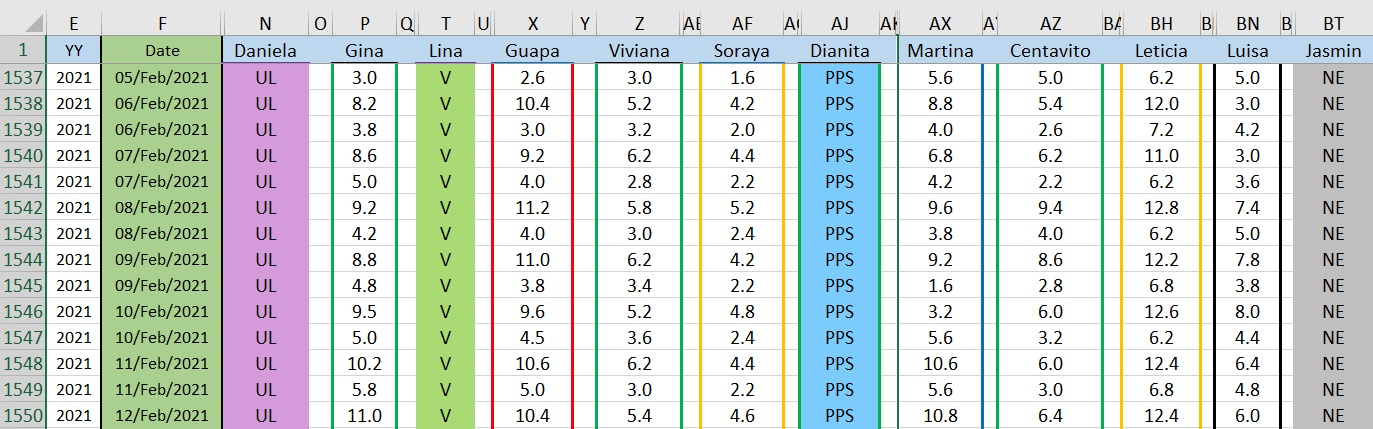
\includegraphics[scale=0.45]{img/dfcolorpartos.jpg}
	 \end{center}
	 \caption{Clasificación de datos por \#Parto para cada vaca. \label{colorpartospng}}
\end{figure}

En la figura anterior se puede observar que la clasificación de los partos se realiza con base en la estructuración de datos tanto categóricos como numéricos. Esto con el objetivo de diferenciar de manera visual entre un periodo de producción de leche a un periodo de secado (Casilla blanca con borde de color y casillas coloreadas de color azul respectivamente). No obstante una vez realizada la clasificación, selección y agrupación de datos; las matrices usadas en los análisis posteriores con algoritmos en Matlab, manejan la estructuración numérica descrita en la sub-sección anterior.\\

Percatese que al tener 6 grupos de partos en el CA-SENA-POP, se utiliza un código de colores para la clasificación de producción por \# de Parto, siendo esta la siguiente:

% Please add the following required packages to your document preamble:
% \usepackage{graphicx}
% \usepackage[table,xcdraw]{xcolor}
% If you use beamer only pass "xcolor=table" option, i.e. \documentclass[xcolor=table]{beamer}
\begin{table}[H]
\centering
\caption{Código de colores por número de parto}
\label{colorpartos}
\resizebox{\textwidth}{!}{%
\begin{tabular}{|
>{\columncolor[HTML]{FFCE93}}c |
>{\columncolor[HTML]{000000}}c |
>{\columncolor[HTML]{1122C6}}c |
>{\columncolor[HTML]{32CB00}}c |
>{\columncolor[HTML]{FFFE65}}c |
>{\columncolor[HTML]{EF3B3B}}c |
>{\columncolor[HTML]{AD71EB}}c |}
\hline
\textit{\textbf{\begin{tabular}[c]{@{}c@{}}Color del\\  borde\end{tabular}}} &
  {\color[HTML]{FFFFFF} \textit{\textbf{Negro}}} &
  {\color[HTML]{FFFFFF} \textit{\textbf{Azul}}} &
  \textit{\textbf{Verde}} &
  \textit{\textbf{Amarillo}} &
  \textit{\textbf{Rojo}} &
  \textit{\textbf{Morado}} \\ \hline
\textit{\textbf{\begin{tabular}[c]{@{}c@{}}\# de \\ Parto\end{tabular}}} &
  \cellcolor[HTML]{C0C0C0}\textit{\textbf{1}} &
  \cellcolor[HTML]{A3E1F3}\textit{\textbf{2}} &
  \cellcolor[HTML]{A1DA8E}\textit{\textbf{3}} &
  \cellcolor[HTML]{FFFFC7}\textit{\textbf{4}} &
  \cellcolor[HTML]{F39E9E}\textit{\textbf{5}} &
  \cellcolor[HTML]{B791DE}\textit{\textbf{6}} \\ \hline
\end{tabular}%
}
\end{table}

Así pues, se obtienen 6 grupos de un tamaño variable de vacas para cada número de parto. Esta clasificación se puede observar en la tabla \ref{porpartos}. % la tabla gigante de colores que no se deja poner label

\subsubsection{Selección de Datos}

Una de las primeras observaciones obtenidas al realizar la agrupación por partos; es que los datos existentes que han sido agrupados no poseen igual cantidad de datos para cada res. Esto se produce dado que los partos varían en cuestión de duración para cada animal. En primera instancia esto no debería suponer un problema significativo, pues en caso que los partos posean una ligera variabilidad de muestras; bastaría con ``rellenar'' los datos faltantes con ceros o con imputación de datos como la media o la moda; ó por otra parte, bastaría con realizar una agrupación con igual cantidad de muestras.\\

Sin embargo, esta contra medida no puede ser llevada a cabo en razón de que los datos existentes facilitan la agrupación por partos, mas no garantiza que los datos de un parto en específico se encuentren disponibles en su totalidad. En otras palabras, muchos de los datos que se tienen para cada parto son datos de inicio de producción o finalización de producción de leche de las terneras, tanto para las que fallecen, para las que se venden, así como también, para las que a fecha del 31 de Diciembre del 2018 ya se encontraban en periodo productivo.\\

Si se realiza una representación visual individual de los datos, se puede observar claramente que algunas reses tienen muy pocos datos, lo que ``recargaría'' la distribución hacia los extremos, dificultando su análisis descriptivo. Por otra parte, si se hace un contraste de datos teniendo como punto de referencia el inicio de la producción o su finalización en el periodo de secado, la tabla de registros permite evidenciar el desbalance que manifiestan los datos:

\begin{figure}[H]
	 \begin{center}
	 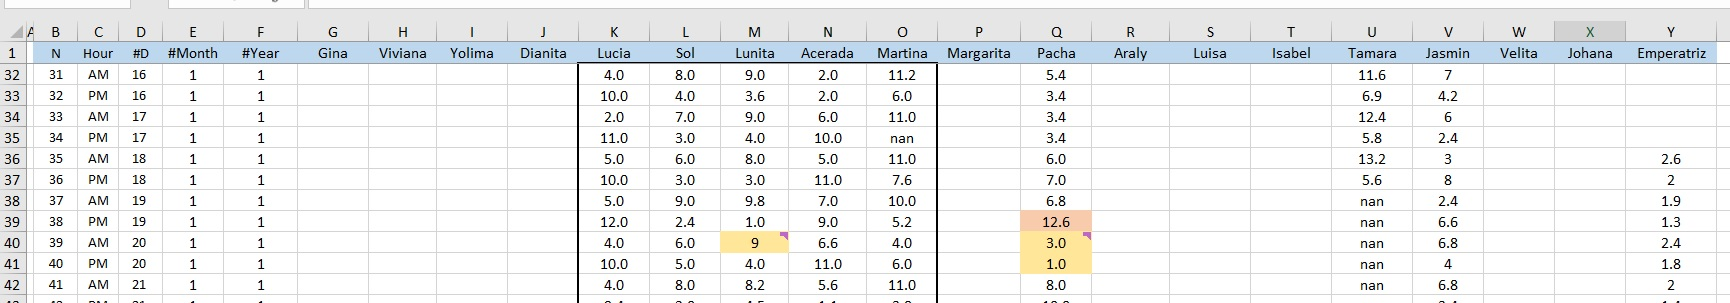
\includegraphics[scale=0.34]{img/partosincompletos.jpg}
	 \end{center}
	 \caption{Desbalance de datos en agrupación inicial por partos. \label{partosincompletospng}}
\end{figure}

En la figura anterior, se evidencia claramente el desbalance mencionado. Si se observan mas a fondo los datos presentes en el archivo de Excel; 13 de las 19 reses cuentan con menos de la mitad de muestras de producción lechera tras haber parido por primera vez. Solo una de ellas, manifiesta un exceso de registros antes de entrar en periodo de secado; y 5 mamíferos restantes aparentan tener la cantidad de muestras suficientes para representar el grupo de vacas primíparas. Las 5 vacas en cuestión son ``Lucia'', ``Sol'', ``Lunita'', ``Acerada'' y ``Martina''.\\

Finalmente, aunque todas las reses cuentan con la misma cantidad de datos, se procede a seleccionar únicamente a 3 de ellas que coinciden en el inicio y finalización de la producción de leche (``Sol'', ``Lunita'', ``Acerada''). Mientras que las otras 2; a pesar de tener la misma cantidad de muestras, presentan desfases en el inicio y finalización de la etapa productiva (Lucia y Martina). De esta forma, se puede generar la primera representación visual de los datos mediante un gráfico de dispersión, tal y como se observa en la  figura \ref{scatterparto1png}.

\begin{figure}[H]
	 \begin{center}
	 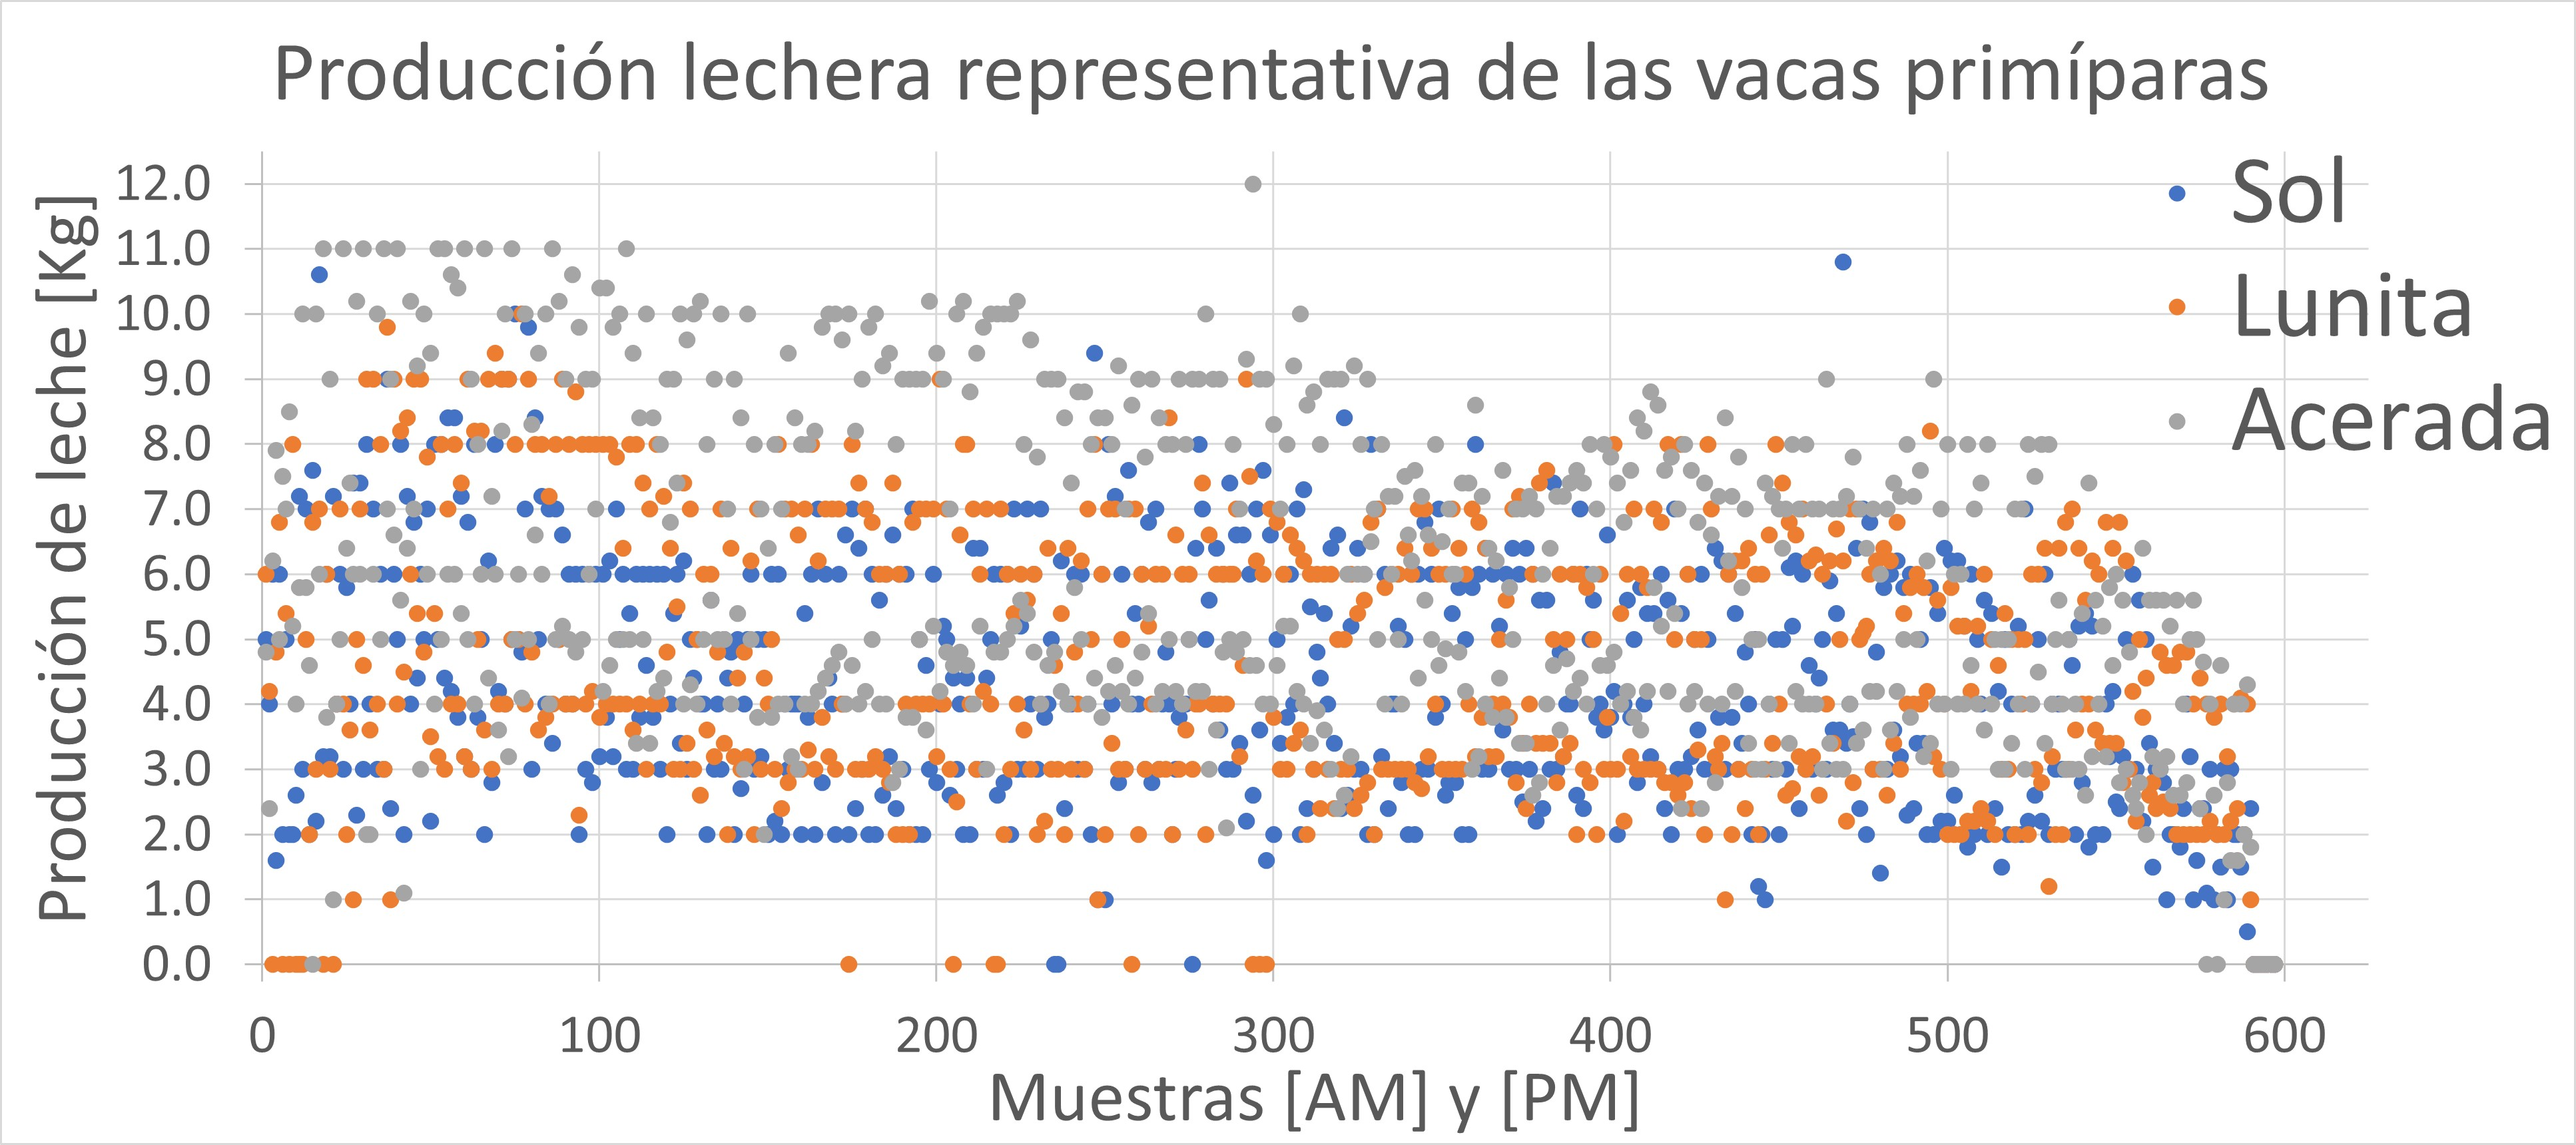
\includegraphics[scale=0.452]{img/scatterparto1.jpg}
	 \end{center}
	 \caption{Gráfico de dispersión para representar la producción lechera de las vacas primíparas. \label{scatterparto1png}}
\end{figure}

\subsubsection{Agrupación de Datos}

El resultado obtenido tras realizar la primer representación visual de datos da un idea de cómo no se deben utilizar los datos para los análisis matemáticos. Pues se observa que al tener muestras matutinas y vespertinas juntas, no se logran diferenciar los datos correspondientes a cada intervalo. Además, el intervalo de tiempo es de 305 días aproximadamente y al manejar ambos tipos de muestras, se tiene un total de 610 datos en el eje horizontal. Por ende, como medida inicial, se opta por realizar un análisis independiente para las muestras obtenidas en diferentes horas del día, procediendo con una representación individual como se observa a continuación:

\begin{figure}[H]
	 \begin{center}
	 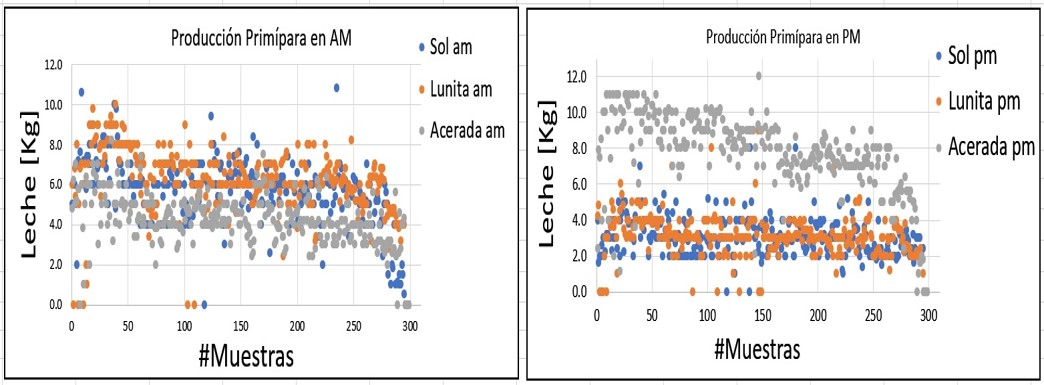
\includegraphics[scale=0.575]{img/desfaseAMPM.jpg}
	 \end{center}
	 \caption{Gráfico de dispersión para Muestras matutinas y vespertinas. \label{desfaseAMPMpng}}
\end{figure}

En primera instancia parece que la gráfica anterior no presenta ningún inconveniente, a pesar de ello, se puede notar un leve desajuste entre los valores vespertinos; pues los valores de la res denominada como ``Acerada'', muestran una lejanía con los otros datos en el horario de la tarde. Esto genera ciertas inquietudes teniendo en cuenta que las muestras matutinas tienden a ser mayores que las muestras vespertinas para la mayoría de las reses de este estudio. En virtud de que el lapso que existe entre una muestra matutina con una vespertina en un mismo día es de aproximadamente 10 horas; mientras que el lapso entre una muestra vespertina y una muestra matutina es de aproximadamente 14 horas; no sería de extrañar que al tener mayor tiempo de recuperación, se le pueda extraer mayor cantidad de leche a la vaca.

Lo anterior se presta para realizar nuevamente una corroboración de los datos con los datos manuales existentes y la tabla de datos de la estructuración inicial; con lo que se observa que al realizar la ``alineación'' de datos tras la agrupación por partos; los datos matutinos de la res en cuestión han quedado ``alineados'' con los datos vespertinos de las otras reses. Esto quiere decir que la figura \ref{desfaseAMPMpng} debe cambiarse por la figura \ref{AMPMsindesfasepng}:


\begin{figure}[H]
	 \begin{center}
	 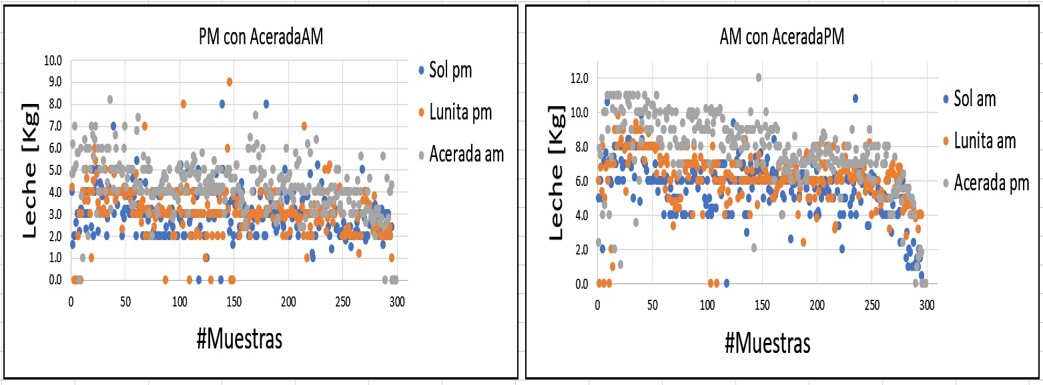
\includegraphics[scale=0.5835]{img/AMPMsindesfase.jpg}
	 \end{center}
	 \caption{Gráfico de dispersión para Muestras matutinas y vespertinas. \label{AMPMsindesfasepng}}
\end{figure}


De acuerdo con la situación anterior, se concluye que realizar un análisis por franja horaria puede llevar a errores futuros o a reincidentes corroboraciones de datos, siendo esto último una tarea agobiante para el caso de estudio; por lo que se decide considerar únicamente análisis con la producción neta diaria de cada animal. De esta forma se repite el proceso para los otros grupos de partos obteniéndose los gráficos de dispersión de la figura \ref{svnetaspng} y obteniéndose un conjunto total de 28 reses para análisis futuros; que se puede observar en la tabla \ref{porpartosfin}.

% Please add the following required packages to your document preamble:
% \usepackage{multirow}
% \usepackage{graphicx}
% \usepackage[table,xcdraw]{xcolor}
% If you use beamer only pass "xcolor=table" option, i.e. \documentclass[xcolor=table]{beamer}
%=======================================================
% Please add the following required packages to your document preamble:
% \usepackage{multirow}
% \usepackage{graphicx}
% \usepackage[table,xcdraw]{xcolor}
% If you use beamer only pass "xcolor=table" option, i.e. \documentclass[xcolor=table]{beamer}
% Please add the following required packages to your document preamble:
% \usepackage{multirow}
% \usepackage{graphicx}
% \usepackage[table,xcdraw]{xcolor}
% If you use beamer only pass "xcolor=table" option, i.e. \documentclass[xcolor=table]{beamer}
\begin{table}[H]
\centering
\caption{Agrupación final de vacas por \# de partos}
\label{porpartosfin}
\resizebox{\textwidth}{!}{%
\begin{tabular}{|
>{\columncolor[HTML]{FFCE93}}c |
>{\columncolor[HTML]{C0C0C0}}c |
>{\columncolor[HTML]{A3E1F3}}c 
>{\columncolor[HTML]{A3E1F3}}c |
>{\columncolor[HTML]{A1DA8E}}c 
>{\columncolor[HTML]{A1DA8E}}c |
>{\columncolor[HTML]{FFFFC7}}c 
>{\columncolor[HTML]{FFFFC7}}c |
>{\columncolor[HTML]{F39E9E}}c |
>{\columncolor[HTML]{B791DE}}c |}
\hline
\textit{\textbf{\# de Parto}} &
  \cellcolor[HTML]{000000}{\color[HTML]{FFFFFF} \textit{\textbf{1}}} &
  \multicolumn{2}{c|}{\cellcolor[HTML]{1122C6}{\color[HTML]{FFFFFF} \textit{\textbf{2}}}} &
  \multicolumn{2}{c|}{\cellcolor[HTML]{32CB00}\textit{\textbf{3}}} &
  \multicolumn{2}{c|}{\cellcolor[HTML]{FFFE65}\textit{\textbf{4}}} &
  \cellcolor[HTML]{EF3B3B}\textit{\textbf{5}} &
  \cellcolor[HTML]{AD71EB}\textit{\textbf{6}} \\ \hline
\cellcolor[HTML]{FFCE93} &
  \textit{\textbf{Acerada}} &
  \multicolumn{1}{c|}{\cellcolor[HTML]{A3E1F3}\textit{\textbf{Dianita}}} &
  \textit{\textbf{Pacha}} &
  \multicolumn{1}{c|}{\cellcolor[HTML]{A1DA8E}\textit{\textbf{Fernanda}}} &
  \textit{\textbf{Martina}} &
  \multicolumn{1}{c|}{\cellcolor[HTML]{FFFFC7}\textit{\textbf{Centavito}}} &
  \textit{\textbf{Muchira}} &
  \textit{\textbf{Andrea}} &
  \textit{\textbf{Andrea}} \\ \cline{2-10} 
\cellcolor[HTML]{FFCE93} &
  \textit{\textbf{Lunita}} &
  \multicolumn{1}{c|}{\cellcolor[HTML]{A3E1F3}\textit{\textbf{Gina}}} &
  \textit{\textbf{Sol}} &
  \multicolumn{1}{c|}{\cellcolor[HTML]{A1DA8E}\textit{\textbf{Guapa}}} &
  \textit{\textbf{Morocha}} &
  \multicolumn{1}{c|}{\cellcolor[HTML]{FFFFC7}\textit{\textbf{Dianita}}} &
  \textit{\textbf{Soraya}} &
  \textit{\textbf{Guapa}} &
  \textit{\textbf{Guapa}} \\ \cline{2-10} 
\cellcolor[HTML]{FFCE93} &
  \textit{\textbf{Sol}} &
  \multicolumn{1}{c|}{\cellcolor[HTML]{A3E1F3}\textit{\textbf{Juanita}}} &
  \textit{\textbf{Viviana}} &
  \multicolumn{1}{c|}{\cellcolor[HTML]{A1DA8E}\textit{\textbf{Juanita}}} &
  \textit{\textbf{Sol}} &
  \multicolumn{1}{c|}{\cellcolor[HTML]{FFFFC7}\textit{\textbf{Leticia}}} &
  \textit{\textbf{Viviana}} &
  \textit{\textbf{}} &
  \textit{\textbf{}} \\ \cline{2-10} 
\multirow{-4}{*}{\cellcolor[HTML]{FFCE93}\textit{\textbf{\begin{tabular}[c]{@{}c@{}}Vacas \\ participantes\end{tabular}}}} &
  \textit{\textbf{}} &
  \multicolumn{1}{c|}{\cellcolor[HTML]{A3E1F3}\textit{\textbf{Lucia}}} &
  \textit{\textbf{}} &
  \multicolumn{1}{c|}{\cellcolor[HTML]{A1DA8E}\textit{\textbf{Leticia}}} &
  \textit{\textbf{}} &
  \multicolumn{1}{c|}{\cellcolor[HTML]{FFFFC7}\textit{\textbf{Morocha}}} &
  \textit{\textbf{}} &
  \textit{\textbf{}} &
  \textit{\textbf{}} \\ \hline
\end{tabular}%
}
\end{table}
%=======================================================
% Corregir que el parto 4 no salió bien la leyenda >:C

\begin{figure}[H]
	 \begin{center}
	 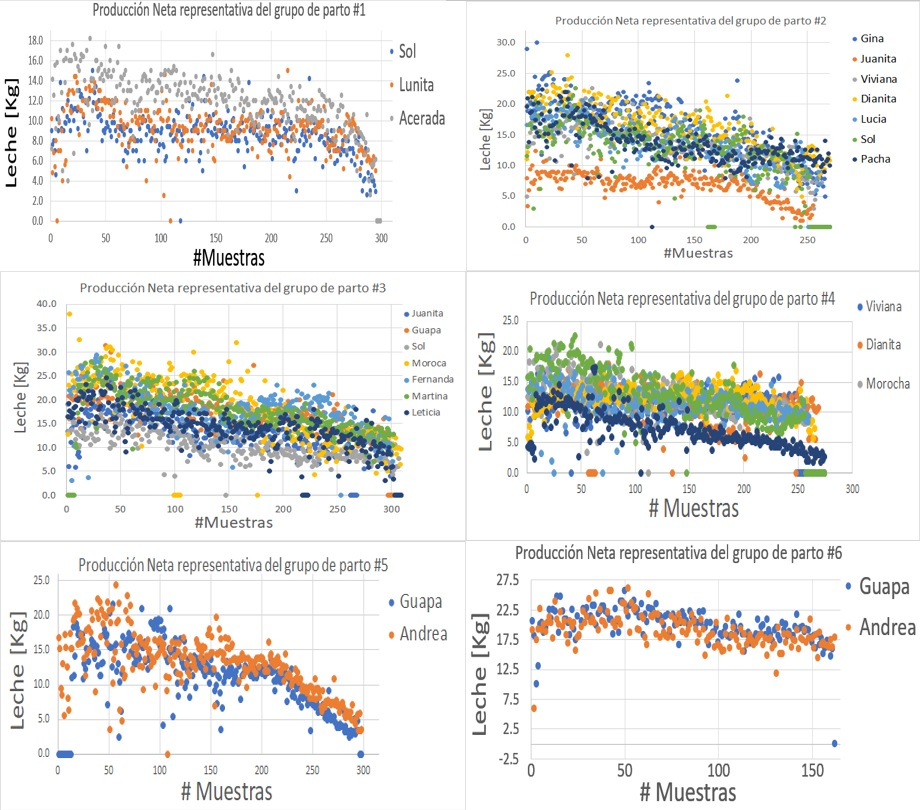
\includegraphics[scale=0.675]{img/svnetas.jpg}
	 \end{center}
	 \caption{Gráfico de dispersión para cada grupo de partos. \label{svnetaspng}}
\end{figure}


% , dando paso en este análisis, que la agrupación de datos de dispersión por partos se le denomine como datos de dispersión neta de ``supervaca'' del parto 1:

% \begin{figure}[H]
% 	 \begin{center}
% 	 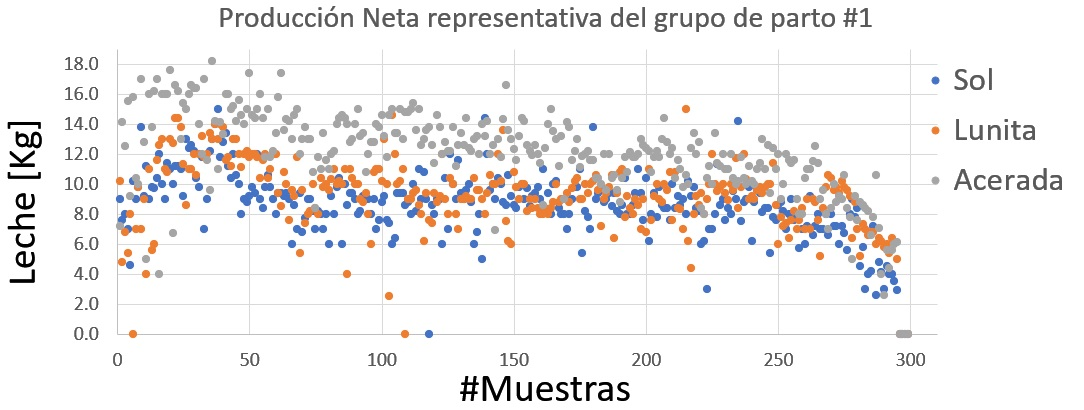
\includegraphics[scale=0.6]{img/svnetap1.jpg}
% 	 \end{center}
% 	 \caption{Gráfico de dispersión para registros de producción neta en vacas primíparas . \label{desfaseAMPMpng}}
% \end{figure}

%================================================================================================
% Please add the following required packages to your document preamble:
% \usepackage{multirow}
% \usepackage{graphicx}
% \usepackage[table,xcdraw]{xcolor}
% If you use beamer only pass "xcolor=table" option, i.e. \documentclass[xcolor=table]{beamer}
% Please add the following required packages to your document preamble:
% \usepackage{multirow}
% \usepackage{graphicx}
% \usepackage[table,xcdraw]{xcolor}
% If you use beamer only pass "xcolor=table" option, i.e. \documentclass[xcolor=table]{beamer}
\begin{table}[H]
\centering
\caption{Agrupación de vacas por \# de partos}
\label{porpartos}
\resizebox{\textwidth}{!}{%
\begin{tabular}{|c|ccccc|}
\hline
\rowcolor[HTML]{FFCE93} 
\textit{\textbf{\begin{tabular}[c]{@{}c@{}}\# de \\ Parto\end{tabular}}} &
  \multicolumn{5}{c|}{\cellcolor[HTML]{FFCE93}\textit{\textbf{\begin{tabular}[c]{@{}c@{}}Vacas \\ participantes\end{tabular}}}} \\ \hline
\rowcolor[HTML]{C0C0C0} 
\cellcolor[HTML]{000000}{\color[HTML]{FFFFFF} } &
  \multicolumn{1}{c|}{\cellcolor[HTML]{C0C0C0}\textit{\textbf{Gina}}} &
  \multicolumn{1}{c|}{\cellcolor[HTML]{C0C0C0}\textit{\textbf{Viviana}}} &
  \multicolumn{1}{c|}{\cellcolor[HTML]{C0C0C0}\textit{\textbf{Yolima}}} &
  \multicolumn{1}{c|}{\cellcolor[HTML]{C0C0C0}\textit{\textbf{Dianita}}} &
  \textit{\textbf{Lucia}} \\ \cline{2-6} 
\rowcolor[HTML]{C0C0C0} 
\cellcolor[HTML]{000000}{\color[HTML]{FFFFFF} } &
  \multicolumn{1}{c|}{\cellcolor[HTML]{C0C0C0}\textit{\textbf{Pacha}}} &
  \multicolumn{1}{c|}{\cellcolor[HTML]{C0C0C0}\textit{\textbf{Araly}}} &
  \multicolumn{1}{c|}{\cellcolor[HTML]{C0C0C0}\textit{\textbf{Luisa}}} &
  \multicolumn{1}{c|}{\cellcolor[HTML]{C0C0C0}\textit{\textbf{Isabel}}} &
  \textit{\textbf{Tamara}} \\ \cline{2-6} 
\rowcolor[HTML]{C0C0C0} 
\cellcolor[HTML]{000000}{\color[HTML]{FFFFFF} } &
  \multicolumn{1}{c|}{\cellcolor[HTML]{C0C0C0}\textit{\textbf{Sol}}} &
  \multicolumn{1}{c|}{\cellcolor[HTML]{C0C0C0}\textit{\textbf{Lunita}}} &
  \multicolumn{1}{c|}{\cellcolor[HTML]{C0C0C0}\textit{\textbf{Acerada}}} &
  \multicolumn{1}{c|}{\cellcolor[HTML]{C0C0C0}\textit{\textbf{Martina}}} &
  \textit{\textbf{Margarita}} \\ \cline{2-6} 
\rowcolor[HTML]{C0C0C0} 
\multirow{-4}{*}{\cellcolor[HTML]{000000}{\color[HTML]{FFFFFF} \textit{\textbf{1}}}} &
  \multicolumn{1}{c|}{\cellcolor[HTML]{C0C0C0}\textit{\textbf{Jasmin}}} &
  \multicolumn{1}{c|}{\cellcolor[HTML]{C0C0C0}\textit{\textbf{Velita}}} &
  \multicolumn{1}{c|}{\cellcolor[HTML]{C0C0C0}\textit{\textbf{Johana}}} &
  \multicolumn{1}{c|}{\cellcolor[HTML]{C0C0C0}\textit{\textbf{Emperatriz}}} &
  \textit{\textbf{}} \\ \hline
\rowcolor[HTML]{A3E1F3} 
\cellcolor[HTML]{1122C6}{\color[HTML]{FFFFFF} } &
  \multicolumn{1}{c|}{\cellcolor[HTML]{A3E1F3}\textit{\textbf{Gina}}} &
  \multicolumn{1}{c|}{\cellcolor[HTML]{A3E1F3}\textit{\textbf{Juanita}}} &
  \multicolumn{1}{c|}{\cellcolor[HTML]{A3E1F3}\textit{\textbf{Guapa}}} &
  \multicolumn{1}{c|}{\cellcolor[HTML]{A3E1F3}\textit{\textbf{Viviana}}} &
  \textit{\textbf{}} \\ \cline{2-6} 
\rowcolor[HTML]{A3E1F3} 
\cellcolor[HTML]{1122C6}{\color[HTML]{FFFFFF} } &
  \multicolumn{1}{c|}{\cellcolor[HTML]{A3E1F3}\textit{\textbf{Fernanda}}} &
  \multicolumn{1}{c|}{\cellcolor[HTML]{A3E1F3}\textit{\textbf{Acerada}}} &
  \multicolumn{1}{c|}{\cellcolor[HTML]{A3E1F3}\textit{\textbf{Martina}}} &
  \multicolumn{1}{c|}{\cellcolor[HTML]{A3E1F3}\textit{\textbf{Centavito}}} &
  \textit{\textbf{}} \\ \cline{2-6} 
\rowcolor[HTML]{A3E1F3} 
\cellcolor[HTML]{1122C6}{\color[HTML]{FFFFFF} } &
  \multicolumn{1}{c|}{\cellcolor[HTML]{A3E1F3}\textit{\textbf{Andrea}}} &
  \multicolumn{1}{c|}{\cellcolor[HTML]{A3E1F3}\textit{\textbf{Yolima}}} &
  \multicolumn{1}{c|}{\cellcolor[HTML]{A3E1F3}\textit{\textbf{Soraya}}} &
  \multicolumn{1}{c|}{\cellcolor[HTML]{A3E1F3}\textit{\textbf{Danna}}} &
  \textit{\textbf{}} \\ \cline{2-6} 
\rowcolor[HTML]{A3E1F3} 
\cellcolor[HTML]{1122C6}{\color[HTML]{FFFFFF} } &
  \multicolumn{1}{c|}{\cellcolor[HTML]{A3E1F3}\textit{\textbf{Muchira}}} &
  \multicolumn{1}{c|}{\cellcolor[HTML]{A3E1F3}\textit{\textbf{Margarita}}} &
  \multicolumn{1}{c|}{\cellcolor[HTML]{A3E1F3}\textit{\textbf{Romina}}} &
  \multicolumn{1}{c|}{\cellcolor[HTML]{A3E1F3}\textit{\textbf{Pacha}}} &
  \textit{\textbf{}} \\ \cline{2-6} 
\rowcolor[HTML]{A3E1F3} 
\cellcolor[HTML]{1122C6}{\color[HTML]{FFFFFF} } &
  \multicolumn{1}{c|}{\cellcolor[HTML]{A3E1F3}\textit{\textbf{Dianita}}} &
  \multicolumn{1}{c|}{\cellcolor[HTML]{A3E1F3}\textit{\textbf{Lucia}}} &
  \multicolumn{1}{c|}{\cellcolor[HTML]{A3E1F3}\textit{\textbf{Sol}}} &
  \multicolumn{1}{c|}{\cellcolor[HTML]{A3E1F3}\textit{\textbf{Morocha}}} &
  \textit{\textbf{Lunita}} \\ \cline{2-6} 
\rowcolor[HTML]{A3E1F3} 
\multirow{-6}{*}{\cellcolor[HTML]{1122C6}{\color[HTML]{FFFFFF} \textit{\textbf{2}}}} &
  \multicolumn{1}{c|}{\cellcolor[HTML]{A3E1F3}\textit{\textbf{Araly}}} &
  \multicolumn{1}{c|}{\cellcolor[HTML]{A3E1F3}\textit{\textbf{Luisa}}} &
  \multicolumn{1}{c|}{\cellcolor[HTML]{A3E1F3}\textit{\textbf{Isabel}}} &
  \multicolumn{1}{c|}{\cellcolor[HTML]{A3E1F3}\textit{\textbf{Tamara}}} &
  \textit{\textbf{Johana}} \\ \hline
\rowcolor[HTML]{A1DA8E} 
\cellcolor[HTML]{32CB00} &
  \multicolumn{1}{c|}{\cellcolor[HTML]{A1DA8E}\textit{\textbf{Gina}}} &
  \multicolumn{1}{c|}{\cellcolor[HTML]{A1DA8E}\textit{\textbf{Juanita}}} &
  \multicolumn{1}{c|}{\cellcolor[HTML]{A1DA8E}\textit{\textbf{Guapa}}} &
  \multicolumn{1}{c|}{\cellcolor[HTML]{A1DA8E}\textit{\textbf{Viviana}}} &
  \textit{\textbf{Lucia}} \\ \cline{2-6} 
\rowcolor[HTML]{A1DA8E} 
\cellcolor[HTML]{32CB00} &
  \multicolumn{1}{c|}{\cellcolor[HTML]{A1DA8E}\textit{\textbf{Morocha}}} &
  \multicolumn{1}{c|}{\cellcolor[HTML]{A1DA8E}\textit{\textbf{Lunita}}} &
  \multicolumn{1}{c|}{\cellcolor[HTML]{A1DA8E}\textit{\textbf{Fernanda}}} &
  \multicolumn{1}{c|}{\cellcolor[HTML]{A1DA8E}\textit{\textbf{Martina}}} &
  \textit{\textbf{Pacha}} \\ \cline{2-6} 
\rowcolor[HTML]{A1DA8E} 
\cellcolor[HTML]{32CB00} &
  \multicolumn{1}{c|}{\cellcolor[HTML]{A1DA8E}\textit{\textbf{Andrea}}} &
  \multicolumn{1}{c|}{\cellcolor[HTML]{A1DA8E}\textit{\textbf{Yolima}}} &
  \multicolumn{1}{c|}{\cellcolor[HTML]{A1DA8E}\textit{\textbf{Soraya}}} &
  \multicolumn{1}{c|}{\cellcolor[HTML]{A1DA8E}\textit{\textbf{Dianita}}} &
  \textit{\textbf{Sol}} \\ \cline{2-6} 
\rowcolor[HTML]{A1DA8E} 
\multirow{-4}{*}{\cellcolor[HTML]{32CB00}\textit{\textbf{3}}} &
  \multicolumn{1}{c|}{\cellcolor[HTML]{A1DA8E}\textit{\textbf{Centavito}}} &
  \multicolumn{1}{c|}{\cellcolor[HTML]{A1DA8E}\textit{\textbf{Muchira}}} &
  \multicolumn{1}{c|}{\cellcolor[HTML]{A1DA8E}\textit{\textbf{Romina}}} &
  \multicolumn{1}{c|}{\cellcolor[HTML]{A1DA8E}\textit{\textbf{Leticia}}} &
  \textit{\textbf{}} \\ \hline
\rowcolor[HTML]{FFFFC7} 
\cellcolor[HTML]{FFFE65} &
  \multicolumn{1}{c|}{\cellcolor[HTML]{FFFFC7}\textit{\textbf{Guapa}}} &
  \multicolumn{1}{c|}{\cellcolor[HTML]{FFFFC7}\textit{\textbf{Viviana}}} &
  \multicolumn{1}{c|}{\cellcolor[HTML]{FFFFC7}\textit{\textbf{Andrea}}} &
  \multicolumn{1}{c|}{\cellcolor[HTML]{FFFFC7}\textit{\textbf{Yolima}}} &
  \textit{\textbf{}} \\ \cline{2-6} 
\rowcolor[HTML]{FFFFC7} 
\cellcolor[HTML]{FFFE65} &
  \multicolumn{1}{c|}{\cellcolor[HTML]{FFFFC7}\textit{\textbf{Sol}}} &
  \multicolumn{1}{c|}{\cellcolor[HTML]{FFFFC7}\textit{\textbf{Morocha}}} &
  \multicolumn{1}{c|}{\cellcolor[HTML]{FFFFC7}\textit{\textbf{Fernanda}}} &
  \multicolumn{1}{c|}{\cellcolor[HTML]{FFFFC7}\textit{\textbf{Centavito}}} &
  \textit{\textbf{}} \\ \cline{2-6} 
\rowcolor[HTML]{FFFFC7} 
\multirow{-3}{*}{\cellcolor[HTML]{FFFE65}\textit{\textbf{4}}} &
  \multicolumn{1}{c|}{\cellcolor[HTML]{FFFFC7}\textit{\textbf{Soraya}}} &
  \multicolumn{1}{c|}{\cellcolor[HTML]{FFFFC7}\textit{\textbf{Dianita}}} &
  \multicolumn{1}{c|}{\cellcolor[HTML]{FFFFC7}\textit{\textbf{Muchira}}} &
  \multicolumn{1}{c|}{\cellcolor[HTML]{FFFFC7}\textit{\textbf{Leticia}}} &
  \textit{\textbf{}} \\ \hline
\rowcolor[HTML]{F39E9E} 
\cellcolor[HTML]{EF3B3B} &
  \multicolumn{1}{c|}{\cellcolor[HTML]{F39E9E}\textit{\textbf{Nancy}}} &
  \multicolumn{1}{c|}{\cellcolor[HTML]{F39E9E}\textit{\textbf{Guapa}}} &
  \multicolumn{1}{c|}{\cellcolor[HTML]{F39E9E}\textit{\textbf{Andrea}}} &
  \multicolumn{1}{c|}{\cellcolor[HTML]{F39E9E}\textit{\textbf{Soraya}}} &
  \textit{\textbf{}} \\ \cline{2-6} 
\rowcolor[HTML]{F39E9E} 
\multirow{-2}{*}{\cellcolor[HTML]{EF3B3B}\textit{\textbf{5}}} &
  \multicolumn{1}{c|}{\cellcolor[HTML]{F39E9E}\textit{\textbf{Dianita}}} &
  \multicolumn{1}{c|}{\cellcolor[HTML]{F39E9E}\textit{\textbf{Centavito}}} &
  \multicolumn{1}{c|}{\cellcolor[HTML]{F39E9E}\textit{\textbf{Muchira}}} &
  \multicolumn{1}{c|}{\cellcolor[HTML]{F39E9E}\textit{\textbf{Leticia}}} &
  \textit{\textbf{}} \\ \hline
\rowcolor[HTML]{B791DE} 
\cellcolor[HTML]{AD71EB}\textit{\textbf{6}} &
  \multicolumn{1}{c|}{\cellcolor[HTML]{B791DE}\textit{\textbf{Daniela}}} &
  \multicolumn{1}{c|}{\cellcolor[HTML]{B791DE}\textit{\textbf{Lina}}} &
  \multicolumn{1}{c|}{\cellcolor[HTML]{B791DE}\textit{\textbf{Guapa}}} &
  \multicolumn{1}{c|}{\cellcolor[HTML]{B791DE}\textit{\textbf{Andrea}}} &
  \textit{\textbf{}} \\ \hline
\end{tabular}%
}
\end{table}

\pagebreak
\section{Reestructuración de los datos de peso}\label{reestructpeso}

Tal y como se mencionó en la sección \ref{datarecol}, los datos referentes al peso de los animales usados en la producción de leche se encuentran registrados en el software ``TaurusWebs'', y con el objetivo posterior de ser exportados y analizados, debemos realizar la transcripción manual de dichos datos.

\subsection{Reorganización de datos}\label{pocospesos}
Esta transcripción de datos se realiza de tal forma que se mantienen los datos asociados a las fechas especificadas tal y como se puede observar en la figura \ref{dfpesopng}.
\begin{figure}[H]
	 \begin{center}
	 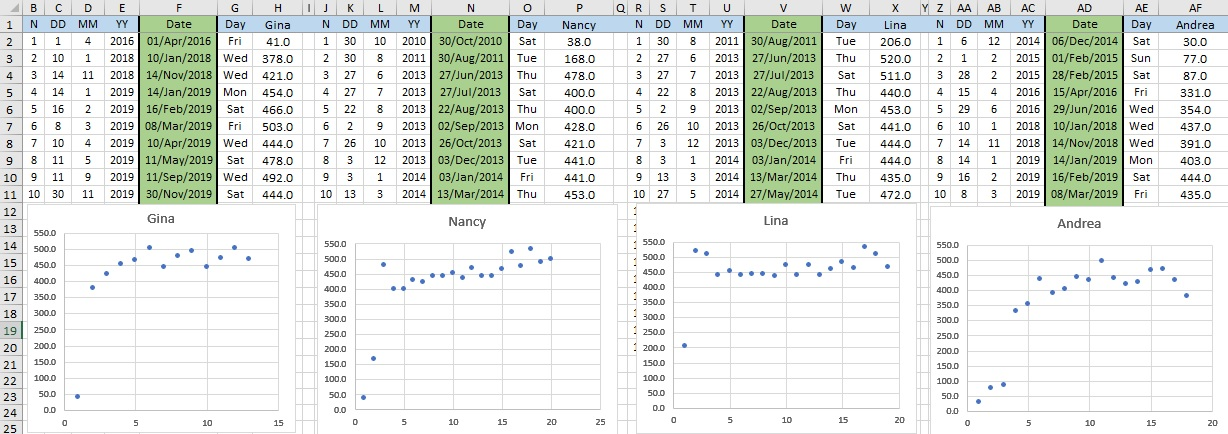
\includegraphics[scale=0.5]{img/dfinicialpeso.jpg}
	 \end{center}
	 \caption{Reorganización inicial de los datos de peso.  \label{dfpesopng}}
\end{figure}

Sin embargo, tras realizar contrastes de fechas de registros de peso con las fechas de registros de leche, se encuentra con que los registros de peso coinciden parcialmente con los registros de leche en un mismo periodo. Esto quiere decir que de los pocos datos existentes respecto al peso, estos deben ser segmentados de acuerdo con el número de parto con el que coinciden las fechas de registro de producción de leche asociadas a la lactancia de ese parto. En función de lo expresado anteriormente, se debe realizar la segmentación de los datos de peso que pertenecen a cada parto (1..6) para cada vaca perteneciente a la tabla \ref{porpartosfin} de la sección anterior.\\


\subsection{Agrupación de datos de peso}
De la tabla \ref{Nporpartos} se tienen 18 vacas diferentes para un total de 28 partos distintos que dependiendo del número de parto se cuenta con una cantidad de muestras distinta (Entre 162 y 309 muestras). Ahora bien, para los análisis algorítmicos en Matlab y/o Python, se requiere que la cantidad de muestras de leche tengan la misma cantidad de muestras para el peso en pro de lograr un análisis por ``Ecuaciones Diferenciales Ordinarias''; por tanto es necesario realizar una interpolación del(los) dato(s) de peso dependiendo de la cantidad de muestras presentes en cada parto.
%=================================================
% Please add the following required packages to your document preamble:
% \usepackage{multirow}
% \usepackage{graphicx}
% \usepackage[table,xcdraw]{xcolor}
% If you use beamer only pass "xcolor=table" option, i.e. \documentclass[xcolor=table]{beamer}
% Please add the following required packages to your document preamble:
% \usepackage{multirow}
% \usepackage{graphicx}
% \usepackage[table,xcdraw]{xcolor}
% If you use beamer only pass "xcolor=table" option, i.e. \documentclass[xcolor=table]{beamer}
\begin{table}[H]
\centering
\caption{Cantidad de muestras para cada vaca de cada parto}
\label{Nporpartos}
\resizebox{\textwidth}{!}{%
\begin{tabular}{|
>{\columncolor[HTML]{FFCE93}}c |
>{\columncolor[HTML]{C0C0C0}}c |
>{\columncolor[HTML]{A3E1F3}}c 
>{\columncolor[HTML]{A3E1F3}}c |
>{\columncolor[HTML]{A1DA8E}}c 
>{\columncolor[HTML]{A1DA8E}}c |
>{\columncolor[HTML]{FFFFC7}}c 
>{\columncolor[HTML]{FFFFC7}}c |
>{\columncolor[HTML]{F39E9E}}c |
>{\columncolor[HTML]{B791DE}}c |}
\hline
\textbf{\# de Parto} &
  \cellcolor[HTML]{343434}{\color[HTML]{FFFFFF} \textit{\textbf{1}}} &
  \multicolumn{2}{c|}{\cellcolor[HTML]{1122C6}{\color[HTML]{FFFFFF} \textit{\textbf{2}}}} &
  \multicolumn{2}{c|}{\cellcolor[HTML]{32CB00}\textit{\textbf{3}}} &
  \multicolumn{2}{c|}{\cellcolor[HTML]{FFFE65}\textit{\textbf{4}}} &
  \cellcolor[HTML]{EF3B3B}\textit{\textbf{5}} &
  \cellcolor[HTML]{AD71EB}\textit{\textbf{6}} \\ \hline
\textit{\textbf{\# de Muestras}} &
  \textbf{299} &
  \multicolumn{2}{c|}{\cellcolor[HTML]{A3E1F3}\textbf{288}} &
  \multicolumn{2}{c|}{\cellcolor[HTML]{A1DA8E}\textbf{309}} &
  \multicolumn{2}{c|}{\cellcolor[HTML]{FFFFC7}\textbf{274}} &
  \textbf{298} &
  \textbf{162} \\ \hline
\cellcolor[HTML]{FFCE93} &
  \textit{\textbf{Acerada}} &
  \multicolumn{1}{c|}{\cellcolor[HTML]{A3E1F3}\textit{\textbf{Dianita}}} &
  \textit{\textbf{Pacha}} &
  \multicolumn{1}{c|}{\cellcolor[HTML]{A1DA8E}\textit{\textbf{Fernanda}}} &
  \textit{\textbf{Martina}} &
  \multicolumn{1}{c|}{\cellcolor[HTML]{FFFFC7}\textit{\textbf{Centavito}}} &
  \textit{\textbf{Muchira}} &
  \textit{\textbf{Andrea}} &
  \textit{\textbf{Andrea}} \\ \cline{2-10} 
\cellcolor[HTML]{FFCE93} &
  \textit{\textbf{Lunita}} &
  \multicolumn{1}{c|}{\cellcolor[HTML]{A3E1F3}\textit{\textbf{Gina}}} &
  \textit{\textbf{Sol}} &
  \multicolumn{1}{c|}{\cellcolor[HTML]{A1DA8E}\textit{\textbf{Guapa}}} &
  \textit{\textbf{Morocha}} &
  \multicolumn{1}{c|}{\cellcolor[HTML]{FFFFC7}\textit{\textbf{Dianita}}} &
  \textit{\textbf{Soraya}} &
  \textit{\textbf{Guapa}} &
  \textit{\textbf{Guapa}} \\ \cline{2-10} 
\cellcolor[HTML]{FFCE93} &
  \textit{\textbf{Sol}} &
  \multicolumn{1}{c|}{\cellcolor[HTML]{A3E1F3}\textit{\textbf{Juanita}}} &
  \textit{\textbf{Viviana}} &
  \multicolumn{1}{c|}{\cellcolor[HTML]{A1DA8E}\textit{\textbf{Juanita}}} &
  \textit{\textbf{Sol}} &
  \multicolumn{1}{c|}{\cellcolor[HTML]{FFFFC7}\textit{\textbf{Leticia}}} &
  \textit{\textbf{Viviana}} &
  \textit{\textbf{}} &
  \textit{\textbf{}} \\ \cline{2-10} 
\multirow{-4}{*}{\cellcolor[HTML]{FFCE93}\textbf{\begin{tabular}[c]{@{}c@{}}Vacas \\ participantes\end{tabular}}} &
  \textit{\textbf{}} &
  \multicolumn{1}{c|}{\cellcolor[HTML]{A3E1F3}\textit{\textbf{Lucia}}} &
  \textit{\textbf{}} &
  \multicolumn{1}{c|}{\cellcolor[HTML]{A1DA8E}\textit{\textbf{Leticia}}} &
  \textit{\textbf{}} &
  \multicolumn{1}{c|}{\cellcolor[HTML]{FFFFC7}\textit{\textbf{Morocha}}} &
  \textit{\textbf{}} &
  \textit{\textbf{}} &
  \textit{\textbf{}} \\ \hline
\end{tabular}%
}
\end{table}
%=================================================

\subsubsection{Generación de columnas de peso que serán anexadas a los ``dataframes'' de cada uno de los modelos asociados al número de parto modelado}

El método usado para realizar la interpolación entre los datos de peso son las ``Splines Cúbicas'' que varían en tamaño dependiendo de la cantidad de datos presentes en cada parto. Una vez ejecutado el script de Matlab ``InterpPesosPartesEDOs'' (adjunto en este trabajo de grado)' se obtiene el conjunto de arreglos unidimensionales con los tamaños deseados (ver figura \ref{interpesospng}) y se procede a realizar la exportación correspondiente en archivos separados por comas. Posteriormente se procede a agruparlos en ``dataframes'' para su análisis por EDOs en python. Para cada lactancia se tendrá un ``dataframe'' representativo de ese modelo con las columnas de producciones de leche, peso y estiércol producido por cada vaca perteneciente a esa agrupación de lactancia.

\begin{figure}[H]
	 \begin{center}
	 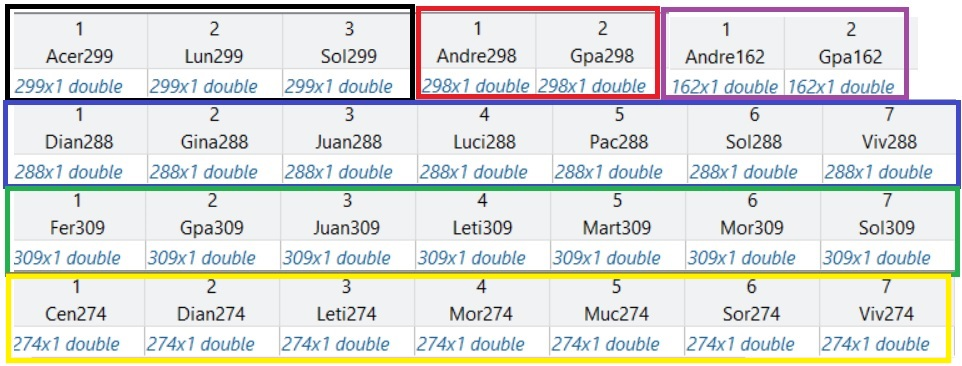
\includegraphics[scale=0.64]{img/InterPesos.jpg}
	 \end{center}
	 \caption{Formato de nombre de columna para conjunto de datos. Varia en cuanto al nombre de la vaca, cantidad de muestras existentes y cantidad de parto. El código de colores se mantiene según la tabla \ref{colorpartos} \label{interpesospng}}
\end{figure}


Llegados a este punto, ya se cuenta con los datos de las 3 variables necesarias (Producción de Leche, Estiércol, Peso) para plantear el (los) modelo(s) por EDOs, descrito en el próximo capitulo.
%================================================================================================
